\documentclass[11pt,a4paper]{article}
\usepackage[utf8]{inputenc}
\usepackage[portuguese]{babel}
\usepackage[T1]{fontenc}
\usepackage{amsmath}
\usepackage{amsfonts}
\usepackage{amssymb}
\usepackage{graphicx}
\usepackage{setspace}

\author{Gustavo Vital\thanks{Mestrando em Economia pela Faculdade de Economia do Porto. Email: gustavovital@id.uff.br}}
\title{Notas sobre o Modelo de Solow\footnote{Baseado em Eric Sims.}}

\onehalfspacing

\begin{document}
\maketitle

O modelo de Solow é ainda hoje um modelo fundamental para a compreensão do crescimento de longo prazo e diferença de renda entre países. Proposto por Robert Solow, mais tarde ganhador do premio nobel de economia, o modelo assume que o crescimento de um país se da fundamentalmente por choques exógenos de tecnologia, dado a função particular de crescimento de longo prazo.

\section{Produção, Consumo, e Investimento}

O modelo de Solow assume que existe uma função de produção agregada tal que seja composta por capital (K) e trabalho (L), sendo esses fatores os responsáveis pela determinação da produção. Ambos, capital e trabalho, são considerados fatores de produção. A distinção fundamental dos dois fatores é: capital é estoque, trabalho é fluxo. \\

O trabalho, ainda em termos de distinção, é dado. Não há nada que se possa fazer para aumentar as horas de trabalho em um dia (por mais que se aumente a carga horária, um dia tem um limite de horas possíveis). O capital -- por outro lado -- é cumulativo. A quantidade de capital num período $t$ influencia \textit{diretamente} a quantidade de capital num período $t+1$.\\

Em termos matemáticos, podemos escrever a função de produção, tal que: seja $K_t$ o estoque de capital no período $t$; e $N_t$ o total de horas de trabalho no período $t$. A função de produção será dada por:
\begin{align}
Y_t &= A_t F(K_t, N_t) 
\end{align}

\noindent
$A_t$ é uma \textbf{variável exógena} que representa produtividade; tecnologia. $F$ é a função de produção ainda não especificada, que relaciona horas de trabalho com capital. A função F($\cdot$) possui as seguintes propriedades $F_K>0$ e $F_N>0$. Isso é, o produto marginal é sempre positivo. Além disso, temos $F_{KK}<0$ e $F_{NN}<0$, retornos decrescente de produção -- quanto mais unidades de capital ou trabalho se possui, menor é a variação do produto em termos de trabalho/capital. assumimos além disso que a função possui retornos constantes de escala. Isso é: $F(\gamma  K_t, \gamma N_t) = \gamma F(K_t, N_t)$. Por fim, assumimos que tanto capital quanto trabalho são necessários para a produção i.e. $F(K_t, 0) = F(0, N_t) = 0$.\\

A fim de apresentar a forma funcional de F($\cdot$), trabalharemos com uma função de produção de formato Cobb-Douglas. Então
\begin{align}
F(K_t, N_t) &= K_t^{\alpha} N_t^{1-\alpha} \quad \text{sendo} \quad 0 < \alpha < 1; 
\end{align}

\noindent
dado o problema acima, a firma buscará otimizar seus lucros ($\Pi_t$) -- produto subtraído de custos e retorno do capital, tal que seu problema de otimização será:
\begin{align}
\max_{K_t, N_t} \Pi_t = A_t F(K_t, N_t) - w_t N_t - R_t K_t \quad ;
\end{align}

\noindent
onde $w_t$ representa o salário pago pelas firmas e $R_t$ o retorno pago pelo capital. As condições de primeira ordem (CPO) são:
\begin{align}
w_t &= A_t F_N(K_t, N_t) \\
R_t &= A_t F_K(K_t, N_t)
\end{align}
\noindent
essas condições dizem que as firmas devem contratar capital e trabalho até o ponto em que os ``benefícios'' marginais se igualam.\\

Além das firmas, devemos representar as famílias desta economia. Bem como de forma simplificada, as famílias ofertam mão de obra e recebem um salário. Além disso, recebem um retorno referente ao capital, de tal forma que $w_t N_t + R_t K_t$ representa a renda da família no período $t$. Ainda, a família pode investir o recebido ou consumir. Sua restrição orçamentária é, então:
\begin{align} \label{eq:restr}
C_t + I_t &= w_t N_t + R_t K_t + \Pi_t
\end{align}

Como já exposto, as firmas operam em retorno constante de escala, então o produto é igual a renda, de forma que $Y_t = w_t N_t + R_t K_t$. Em \ref{eq:restr}, ao considerarmos retorno constantes de escala, temos que $\Pi_t = 0$ e apresenta-se a identidade:
\begin{align} \label{eq:ident}
Y_t = C_t + I_t
\end{align}
\noindent
a evolução do capital por sua vez pode ser apresentada como o estoque de capital no período $t$ não depreciado somado ao investimento do período corrente. Matematicamente:
\begin{align}
K_{t+1} = I_t + (1 - \delta)K_t
\end{align}
\noindent
onde $0<\delta<1$ representa a taxa de depreciação do capital. A equação acima representa a ``lei de movimento'' do capital; mais que isso, ela assume que uma unidade de investimento no período $t$ é totalmente revertido em estoque de capital em $t+1$. Exemplificando a lei de movimento do capital, suponha que $k_t = 10$, a taxa de depreciação do capital é igual a 0.1 ($\delta = 0.1$). Se a produção no período $t$ é 3 ($Y_t = 3$)e o consumo no período $t$ também é igual a 3 ($C_t = 3$) temos que $I_t = 0$, de tal forma que $K_{t+1} = 9$. Se o consumo no período $t$ for igual a 2, significa que o investimento nesse período será igual a 1 e assim o capital no período $t+1$ será igual a 10 novamente. O modelo de Solow, visto dessa forma assume -- então -- que o investimento no período $t$ é uma fração da produção do mesmo período $t$:
\begin{align} \label{eq:s}
I_t = s Y_t \quad \text{sendo} \quad 0 < s < 1;
\end{align} 
\noindent
combinando \ref{eq:s} com \ref{eq:ident} temos:
\begin{align}
C_t = (1-s)Y_t
\end{align}
O modelo de Solow assume dessa forma que a economia pode ser representada pelo consumo corrente num período $t$ e um não-consumo, revertido em investimento, que gera acumulação de capital num período $t+1$. Considera ainda que a quantidade de tempo que uma família passa trabalhando é inelástica ao preço pago pelo trabalho, $w_t$. Assim, o número de horas de trabalho $N_t$ se torna exógeno ao modelo.\footnote{O problema aqui é a ausência da microfundamentação do modelo. A curto prazo as famílias não considerarem a otimização frente a oferta de trabalho não parece fazer muito sentido, a longo prazo entretanto, essa ideia é consistente ao modelo}. O modelo de Solow é caracterizado, dessa forma, pelas seguintes equações:
\begin{align}
Y_t &= A_t F(K_t, N_t)\\ \label{eq:prod}
Y_t &= C_t + I_t\\
K_{t+1} &= I_t + (1-\delta)K_t\\ \label{eq:cap}
I_t &= sY_t\\ \label{eq:inv}
w_t &= A_t F_N(K_t, N_t)\\
R_t &= A_t F_K(K_t, N_t)
\end{align}  
Seis são as equações e seis são as variáveis endógenas. São elas: $Y_t, C_t, I_t, K_{t+1}$, $w_t$ e $R_t$. $K_t, N_t$ e $A_t$ são consideradas \textbf{exógenas} para o modelo, $s$ e $\delta$ são, por sua vez, parâmetros.\\

Podemos ainda combinar as equações \ref{eq:prod}, \ref{eq:cap}, e \ref{eq:inv}, de tal forma que:
\begin{align}
K_{t+1} &= s A_t F(K_t, N_t) + (1-\delta)K_t \label{eq:cap2}
\end{align}
\noindent
A equação \ref{eq:cap2} representa a evolução do capital. Dado o valor exógeno de $k_t, N_t e A_t$, esses compõe o valor futuro do estoque de capital, de forma que $k_{t+1}$ se torna endógeno ao modelo. É vantajoso, entretanto, escrevermos a equação de maneira que essa represente o valor per capita. Assim, dividindo ambos os lados de \ref{eq:cap2} por $N_t$, temos:
\begin{align}
\frac{K_{t+1}}{N_t} &= \frac{s A_t F(K_t, N_t)}{N_t} + \frac{(1-\delta)K_t}{N_t}
\end{align} 
Definimos então a nossa relação em função do capital por trabalhador. Isso é, $k_t \equiv K_t / N_t$. Dado que nossa função de produção possui retornos constantes de escala, podemos escrever a função de produção de forma que:
\begin{align}
\frac{F(K_t, N_t)}{N_t} = F\left(\frac{K_t}{N_t},\frac{N_t}{N_t}\right) = F(k_t, 1);
\end{align}
\noindent
dessa forma, podemos reescrever a equação \ref{eq:cap2} em termos de capital por trabalhador ($f(k_t)\equiv F(k_t, 1)$):
\begin{align}
\frac{K_{t+1}}{N_t} = s A_t f(k_t) + (1-\delta)k_t
\end{align}
A partir desta equação, se multiplicarmos e dividirmos o lado esquerdo por $N_{t+1}$, e considerando que a força de trabalho é exógena e constante em relação a $t, t+1$, temos:
\begin{align*}
\frac{K_{t+1}}{N_t}\frac{N_{t+1}}{N_{t+1}} &= s A_t f(k_t) + (1-\delta)k_t \\
\end{align*}
Em termos de capital per capita, temos a equação central do modelo de Solow:
\begin{align}
k_{t+1} &= s A_t f(k_t) + (1-\delta)k_t \label{eq:central}
\end{align}
\noindent
essa descreve a evolução do capital em termos de trabalhadores, dado a produtividade, a taxa de depreciação do capital e a taxa marginal de investimento. Reescrevendo as equações fundamentais do modelo, em termo de capital por trabalhadores, temos:
\begin{align}
y_t &= Af(k_t)\\
c_t &= (1-s)Af(k_t)\\
i_t &= sAf(k_t)
\end{align}  

\section{Analise Gráfica do Modelo de Solow}
Iremos analisar o modelo de Solow de forma gráfica e matemática. Considere a equação central do modelo de Solow \ref{eq:central}. Podemos graficamente representar essa equação de forma que $k_{t+1}$ se relacione com $k_t$. Se $k_t = 0$, então $k_{t+1}=0$, dado que o capital é uma variável necessária para a produção. Graficamente, isso significa que quando $k_{t+1}$ está no eixo vertical e $k_t$ no eixo horizontal, o gráfico começa na origem. A questão é: como $k_{t+1}$ irá variar, dado uma variação em $k_t$? Afim de uma melhor compreensão da relação capital, tiremos a derivada de $k_{t+1}$ em relação a $k_t$:
\begin{align}
\frac{dk_{t+1}}{dk_t} &= sAf'(k_t) + (1-\delta); \label{eq:slope}
\end{align}
\noindent
a equação \ref{eq:slope} acima representa a inclinação da curva $k_{t+1}$ contra $k_t$. A magnitude da inclinação depende do valor de $k_t$. Ainda, sendo $f'(k_t)$ positivo e $\delta < 1$, a inclinação é positiva, então $k_{t+1}$ cresce em função de $k_t$. Sendo $f''(k_t)<0$, o termo $sAf'(k_t)$ fica cada vez menor conforme $k_t$ aumenta. Vamos assumir mais duas condições\footnote{Essas condições são conhecidas também como ``condições de Inada''}:
\begin{align}\label{eq:inada1}
\lim_{k_t \to 0} f'(k_t) &= \infty\\ \label{eq:inada2}
\lim_{kt \to \infty} f'(k_t) &= 0 
\end{align}	
Em outras palavras, \ref{eq:inada1} diz que o produto marginal do capital é infinito quando não há capital; e \ref{eq:inada2} diz que o produto marginal do capital é zero quando o capital tente ao infinito\footnote{infinitamente grande}.\\

A Figura \ref{fig:eqcentral} representa a relação entre $k_t$ e $k_{t+1}$. A curva começa na origem, e conforme $k_t$ aumenta, $k_{t+1}$ cresce e possui inclinação de $(1-\delta)$. Foi adicionado ao gráfico uma reta de 45 graus, representando $k_t = k_{t+1}$. $k_{t+1}$ inicia com uma inclinação maior que 1 ($\delta < 0$), consequentemente acima da reta de 45 graus e conforme varia\footnote{$\delta < 1$} a inclinação da curva referente a função de acumulação de capital se torna menos inclinada.\\

Eventualmente, dada a inclinação da curva, essa irá cruzar a reta $k_t = k_{t+1}$, no ponto $k_t ^{\ast}$. Esse ponto é conhecido como ``estado estacionário''\footnote{``Steady State''}. \\

\begin{figure}[!h]
\centering
\caption{Grafico da equação central do modelo de Solow} \vspace{2ex}
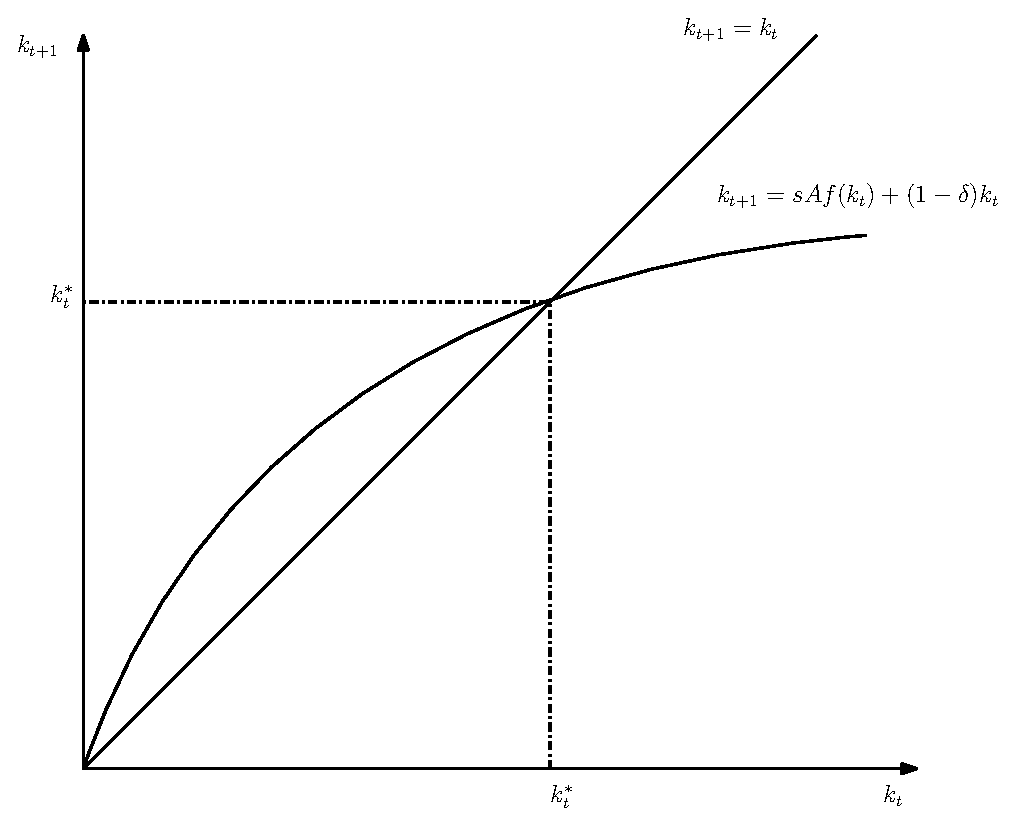
\includegraphics[scale=.5]{solow01.eps}
\label{fig:eqcentral}
\end{figure} 

Normalmente se inclui a reta em 45 graus devido a análise direta do funcionamento do modelo. Isso é, a dinâmica do estoque de capital por trabalhador. Ainda, a reta permite refletir o eixo vertical no eixo horizontal. Por exemplo, suponha que a economia num período $t$ tal que $k_t < k_t ^{\ast}$, dessa forma com estoque de capital abaixo do estoque do estado estacionário. Podemos entender o capital de estoque ``refletindo'' na reta de 45 graus. 

\begin{figure}[!h]
\centering
\caption{Convergência para o estado estacionário ($k_t < k_t ^{\ast}$)} \vspace{2ex}
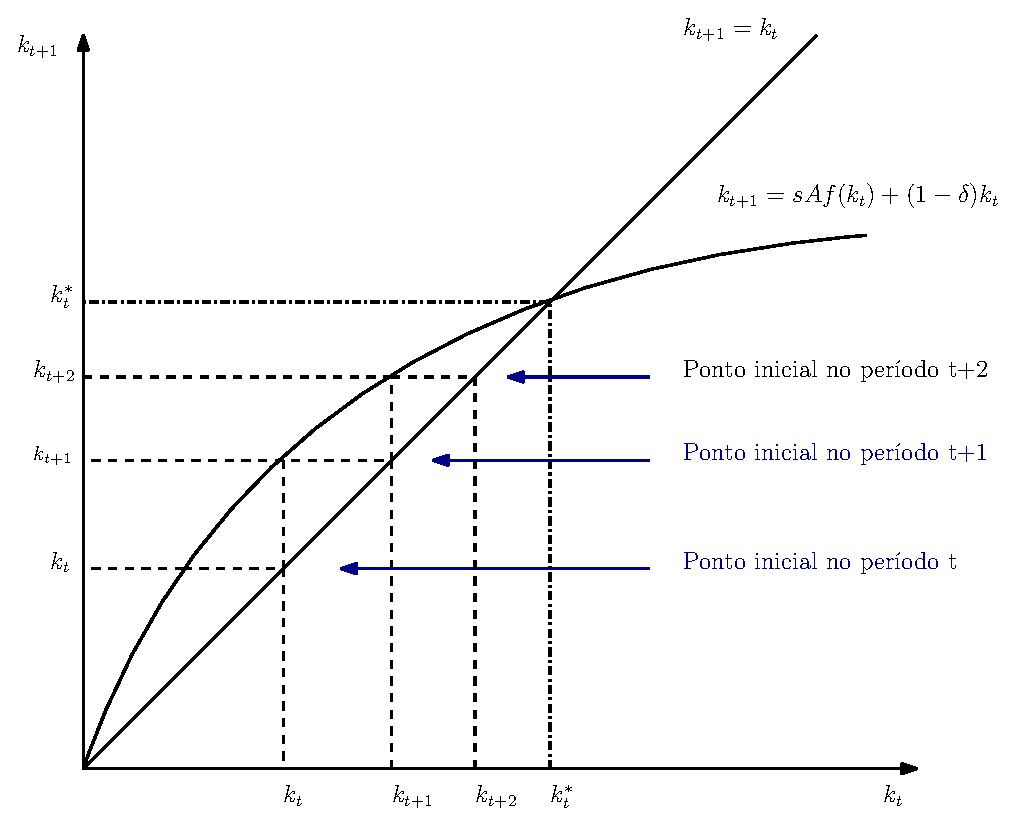
\includegraphics[scale=.5]{solow02.eps}
\label{fig:convergencia}
\end{figure}

O movimento ao estado estacionário acontece pela reflexão na reta que simboliza o estado estacionário. Dado um estoque de capital no período $t$, senão no estado estacionário esse é ``iterado'' entre a curva que representa o estado estacionário e a que representa a equação central do modelo de Solow.\\

A analise feita acima possui um ponto crucial: dado um valor de $k_t$ diferente de zero, o estoque de capital tende a caminhar ao seu estado estacionário. Em outras palavras, o estado estacionário é um ``ponto de atração'' do estoque de capital. Uma vez que o estoque de capital atinge seu estado estacionário este permanece ali, desde que $k_t = k_{t+1}$.\\

O estado estacionário é sempre um ponto de interesse analítico. Não porque uma vez nesse ponto a economia permanece nesse ponto, mas porque independente dos valores iniciais esse é o estado que a economia irá convergir.

\section{A Álgebra do Estado Estacionário A Partir de uma Função Cobb-Douglas de Produção}
Suponhamos agora que a função de produção da economia assume forma funcional de uma Cobb-Douglas. Para resolvermos o modelo no seu estado estacionário temos $k_t = k_{t+1} = k_t ^{\ast}$:
\begin{align}
k_t ^{\ast} = sAk_t ^{\ast \alpha} + (1-\delta)k_t ^{\ast}
\end{align}
\noindent
$k_t ^{\ast}$ pode ser definido como:
\begin{align}
k_t ^{\ast} = \left(\frac{sA}{\delta}\right)^{\frac{1}{1-\alpha}}
\end{align}
A medida em que $s$ e $A$ aumentam, $k_t ^{\ast}$ aumenta. Por sua vez, a medida em que $\delta$ aumenta, $k_t ^{\ast}$ diminui. Isso é, o estoque de capital é inversamente proporcional a taxa de desconto do capital, bem como é proporcional a propensão marginal a investir e a produtividade. Além disso, podemos obter o valor das outras variáveis para o estado estacionário, visto que podemos substituir $k_t ^{\ast}$ nas outras equações, de forma que:
\begin{align}
y^{\ast} &= Ak^{\ast \alpha} \\
c^{\ast} &= (1-s)Ak^{\ast \alpha}\\
i^{\ast} &= sAk^{\ast \alpha} \\
R^{\ast} &= \alpha A k^{\ast \alpha - 1}\\
w^{\ast} &= (1-\alpha)Ak^{\ast \alpha}  
\end{align}
\section{Mudanças em s e Mudanças em A}

Nosso objetivo agora é entender como as variáveis endógenas reagem a mudanças nas variáveis exógenas $s$ e $A$. Vamos considerar inicialmente uma mudança em $s$. Esta, no mundo real, poderia ser vista como uma mudança de política fiscal por exemplo. Suponha inicialmente a economia no estado estacionário, onde $s$ inicial é dado por $s_0$. Então, em $t$, $s_1 > s_0$.\\

Em termos gráficos, um aumento em $s$ desloca a curva da equação central do modelo para cima. Desta forma a economia passa a caminhar para um novo estado estacionário, em que $k_1^{\ast} > k_0^{\ast}$, Figura \ref{fig:convergencia2}  

\begin{figure}[!h]
\centering
\caption{Aumento em $s$, $s_1 > s_0$} \vspace{2ex}
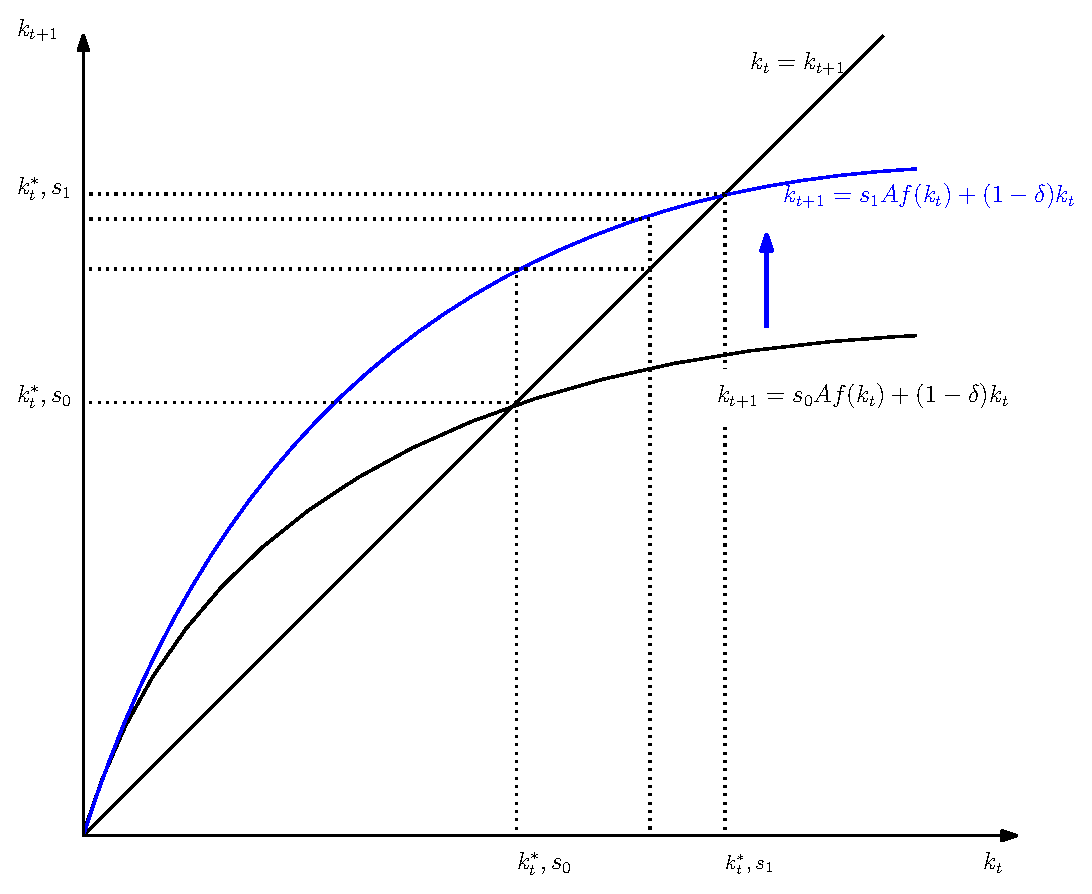
\includegraphics[scale=.5]{solow03.eps}
\label{fig:convergencia2}
\end{figure}

É possível perceber que dado um aumento na propensão marginal a investir, o estoque de capital por trabalhador aumenta. O novo estado estacionário, entretanto, não acontece de uma hora para outra. Como sabemos que $k^\ast , s_1 > k^\ast , s_0$, é interessante observarmos o que ocorre com as outras variáveis endógenas. 

\begin{figure}[!h]
\centering
\caption{Respostas das variáveis endógenas a um aumento em $s$} \vspace{2ex}
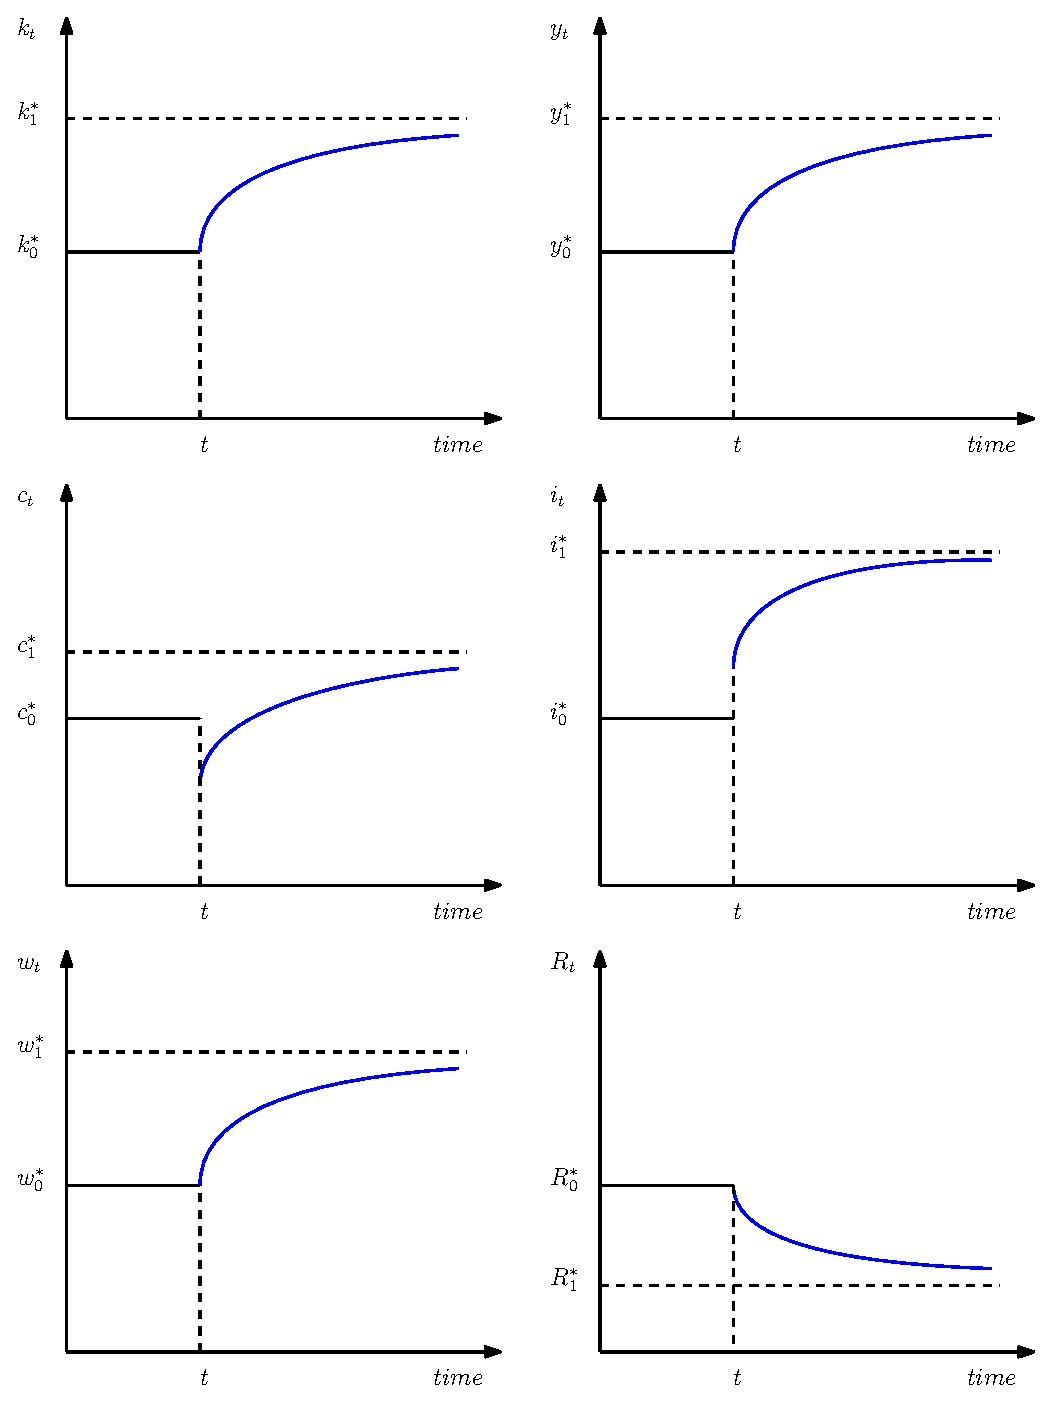
\includegraphics[scale=.72]{solow04.eps}
\label{fig:convergencia3}
\end{figure}

Como mostrado na Figura \ref{fig:convergencia3}, é possível traçarmos a dinâmica de resposta as variáveis endógenas. Dando mais atenção para o comportamento do consumo e do investimento, temos que a representação dessas variáveis no estado estacionário são dadas por:
\begin{align*}
c^{\ast} &= (1-s)Ak^{\ast \alpha}\\
i^{\ast} &= sAk^{\ast \alpha}
\end{align*}
\noindent
de forma que o choque em $s$, propensão marginal a investir afetará \textbf{diretamente} essas duas variáveis no período $t$, enquanto quando comparado com as outras variáveis do modelo, o choque se da ``de forma gradual''. A associação em relação ao consumo e ao investimento parte da identidade de o que não é investido é consumido, e vice-versa. Então, dado um choque positivo em $s$, o consumo irá reduzir a mesma proporção que o investimento aumenta. Como com um aumento em $s$ desloca a economia para um estado estacionário, tal que $k_1^{\ast}>k_0^{\ast}$, o choque negativo no consumo aumenta gradualmente, de forma que $c_1 ^{\ast} > c_0 ^{\ast}$ - dado que o consumo pode ser posto em função do produto. Em relação ao investimento, a lógica é a mesma. Como o investimento é uma função direta do produto, um aumento em $s$ no período $t$ elevará \textbf{imediatamente} o investimento e com o passar do tempo este aumentará mais ainda\footnote{O investimento em $t$ sai do estado estacionário, e seu novo ``Steady State'' se dá no equilíbrio da economia em $k^{\ast}$}.  

\begin{figure}[!h]
\centering
\caption{Trajetória do crescimento pós choque positivo em $s$} \vspace{2ex}
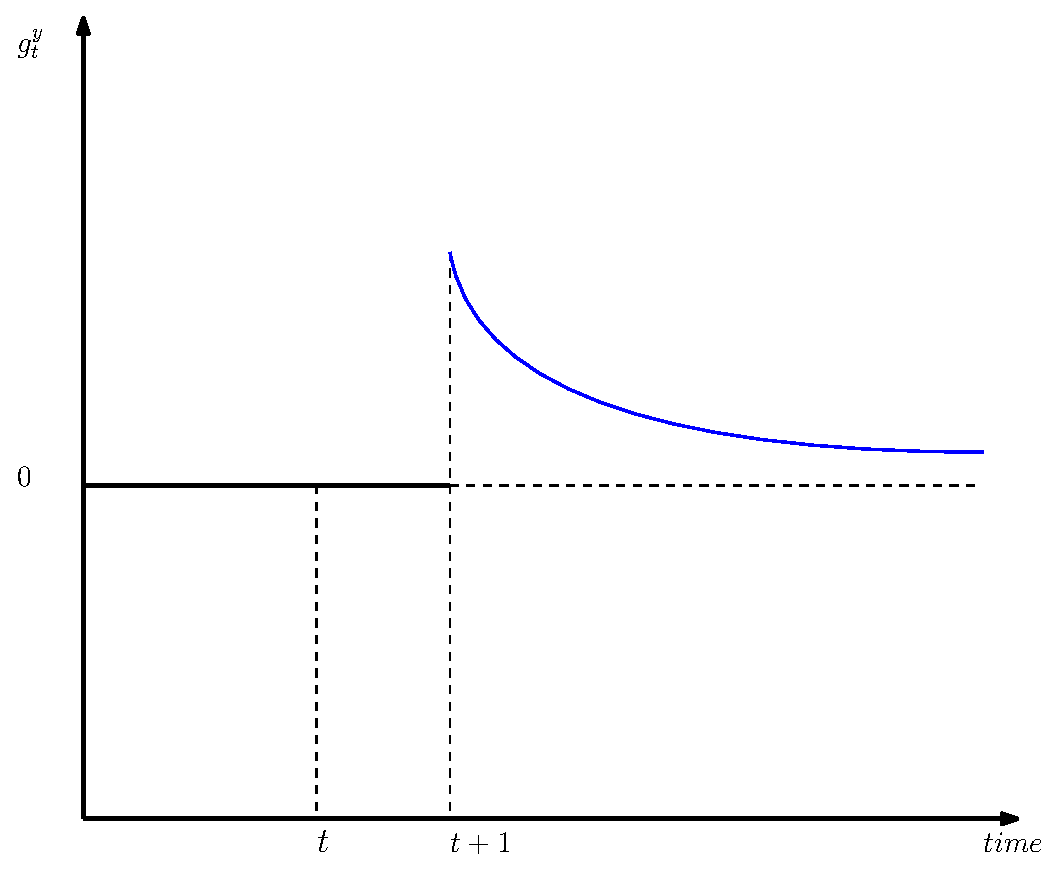
\includegraphics[scale=.4]{solow05.eps}
\label{fig:convergencia4}
\end{figure} 

A Figura \ref{fig:convergencia4} apresenta a convergência da taxa de crescimento da economia pós choque positivo em $s$. Inicialmente há um aumento na taxa de crescimento devido a associação do produto com a propensão a investir. Entretanto, o choque é dissipado até o retorno da taxa de crescimento ao seu estado estacionário.\\

Vamos analisar agora o que acontece com a economia quando há um aumento de produtividade, um aumento em $A$.\\

Diferente do que acontece com um aumento na taxa de investimento, um aumento em $A$ se dá de forma permanente. Suponhamos que num estado inicial estacionário, a produtividade seja representada por $A_0$, dado um choque em $A$, tal que $A_1 > A_0$ os valores futuros de $A$ serão maiores do que $A_0$. Em termos dos efeitos dinâmicos na economia, mostremos antes a representação em função do estoque de capital.  

\begin{figure}[!h]
\centering
\caption{Aumento em $A$, $A_1 > A_0$} \vspace{2ex}
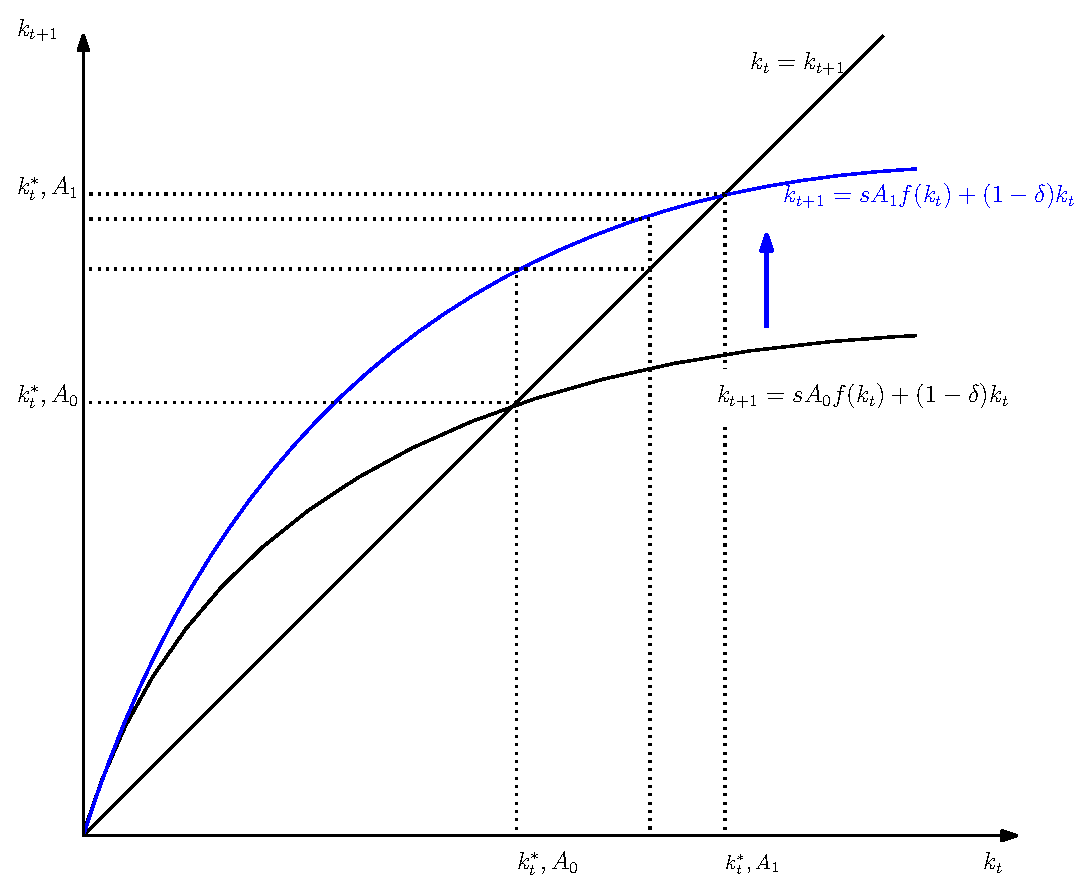
\includegraphics[scale=.5]{solow06.eps}
\label{fig:aumentoa}
\end{figure} 
A Figura \ref{fig:aumentoa}, muito similar a Figura \ref{fig:convergencia2}, representa um aumento na variável $A$, de tal maneira que após o choque de produtividade o estado estacionário da economia passa de $k_t ^{\ast}A_0$ para $k_t ^{\ast}A_1$. Como feito anteriormente, vamos representar o que acontece com as outras variáveis endógenas.

\begin{figure}[!h]
\centering
\caption{Respostas das variáveis endógenas a um aumento em $A$} \vspace{2ex}
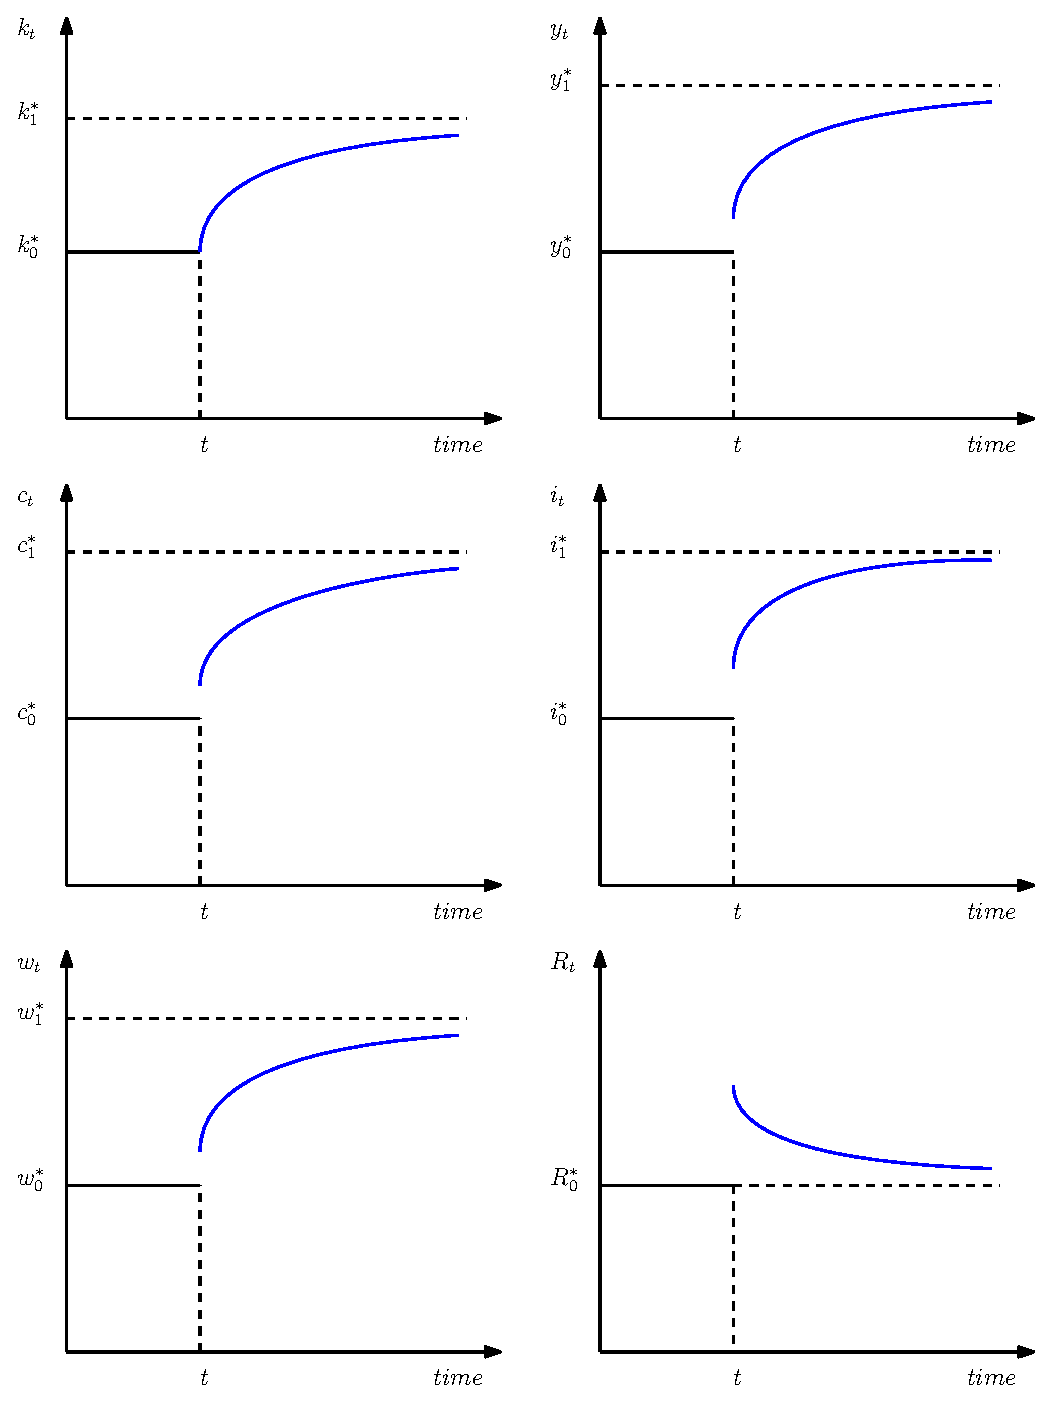
\includegraphics[scale=.72]{solow07.eps}
\label{fig:aumento2a}
\end{figure} 

É interessante perceber que a mudança em $k_t$ é a única que ocorre de forma gradual. Isso porque $k_t$ é a única variável associada diretamente a $A$. A rentabilidade do capital ($R_t$), por sua vez, inicialmente sofre um aumento, devido ao aumento repentino na produtividade marginal do capital e -- então -- de forma gradual tende novamente ao seu estado estacionário. Podemos associar da mesma forma $y_t$. O produto da economia é função do estoque de capital por trabalhador que por sua vez é relacionado a tecnologia, produtividade, da economia.\\

A trajetória do crescimento da economia, por sua vez, é muito similar quando esta sofre um choque em $s$. Devemos, entretanto, nos atentar para o fato de que um aumento da produtividade em $t$ \textbf{afeta a economia já em $t$}. Isso é, não há defasagem como acontece em relação a $s$. O retorno ao estado estacionário, por outro lado, ocorre de maneira semelhante. 

\begin{figure}[!h]
\centering
\caption{Trajetória do crescimento pós choque positivo em $s$} \vspace{2ex}
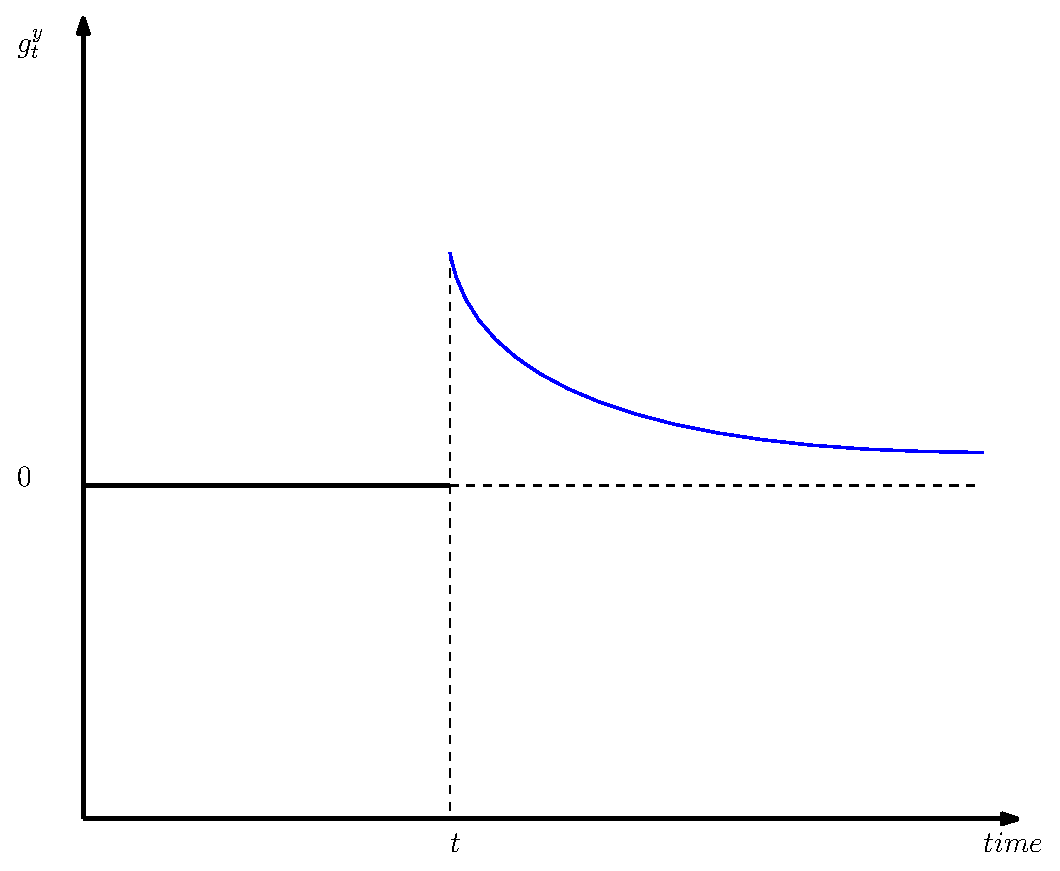
\includegraphics[scale=.5]{solow08.eps}
\label{fig:convergencia5}
\end{figure} 

O questionamento aqui é: dado que pós algum choque de propensão a investir ou tecnológico, a economia retorna ao seu estado estacionário, sua taxa de crescimento é zero -- Figura \ref{fig:convergencia5}. Não é possível, então, manter o crescimento econômico? No modelo básico de Solow, um choque em $s$ não pode ser sustentado por vários períodos de tempo, até pelo próprio possuir um limite $0 < s < 1$. Em relação a tecnologia, é possível, e plausível que choques de produtividade se mantenham por mais de um período de tempo, gerando um crescimento sustentável.

\section{A Regra de Ouro}

Primeiro ponto do modelo: um aumento na taxa de poupança gera um aumento no estoque de capital, bem como no produto da economia. Aumentar a taxa de poupança, entretanto, significa que os agentes estão consumindo menos. O consumo, bem como a poupança é função direta da renda e, no seu estado estacionário:
\begin{align}
c^{\ast} = (1 - s)Af(k^{\ast})
\end{align} 
\noindent
isso é, um aumento de $s$ reduz $(1 - s)$, se $s = 0$, então $f(k^{\ast})=0$, o que não é possível, bem como se $s=1$, o consumo seria nulo, o que também não é possível. Intuitivamente, quando $s$ está próximo de $0$ o consumo diminui, bem como quando $s$ é próximo de $1$ o consumo tende a ser maior. 

\subsection{A Derivação da Regra de Ouro}

Fundamentalmente, a regra de ouro diz que ``a taxa de poupança deve ser tal qual o produto marginal do capital é igual a taxa de depreciação do capital''. Matematizando, o estado estacionário do estoque de capital é dado por:
\begin{align}
sAf(k^{\ast}) = \delta k^{\ast}
\end{align}
derivando a expressão ao seu estado estacionário $s$, temos que:
\begin{align}
sAf'(k^{\ast})dk^{\ast} + Af(k^{\ast})ds = \delta dk^{\ast}
\end{align}
resolvendo para $dk^{\ast}$
\begin{align} 
[sAf'(k^{\ast}) - \delta ]dk^{\ast} = -Af(k^{\ast})ds \label{eq:solvefork}
\end{align}
o consumo $c^{\ast}$ no estado estacionário é dado por:
\begin{align}
c^{\ast} = Af(k^{\ast}) - sAf(k^{\ast})
\end{align}
diferenciando a expressão:
\begin{align}
dc^{\ast} = Af'(k^{\ast})dk^{\ast} - sAf'(k^{\ast})dk^{\ast} - Af(k^{\ast})ds
\end{align}
rearranjando os termos:
\begin{align}
dc^{\ast} = [Af'(k^{\ast}) - sAf'(k^{\ast})]dk^{\ast} - Af(k^{\ast})ds
\end{align}
Conhecendo \ref{eq:solvefork}, sabemos que $Af(k^{\ast})ds = [sAf'(k^{\ast}) - \delta ]dk^{\ast}$
\begin{align}
dc^{\ast} = [Af'(k^{\ast}) - \delta ]dk^{\ast}
\end{align}
dividindo os dois lados por $s$:
\begin{align}
\frac{dc^{\ast}}{ds} = [Af'(k^{\ast}) - \delta ]\frac{dk^{\ast}}{ds}
\end{align}
finalmente, para $s$ maximizar $c^{\ast}$ é o caso de $dc^{\ast}/ds = 0$, desde que $k^{\ast} / ds >0$ só é o caso se:
\begin{align}
Af'(k^{\ast}) = \delta \label{eq:regradeouro}
\end{align}
\noindent
A equação \ref{eq:regradeouro} acima representa a \textbf{regra de ouro}.

\subsection{Análise gráfica}
A representação gráfica da regra de ouro se dá inicialmente pelo comportamento do consumo em relação a taxa de poupança, visto que a própria regra seria $s$ ótimo para a maximização do consumo. A figura \ref{fig:goldenrule} representa a trajetória do consumo frente a taxa de poupança.

\begin{figure}[!h]
\centering
\caption{$s$ e $c^{\ast}$ -- a regra de ouro} \vspace{2ex}
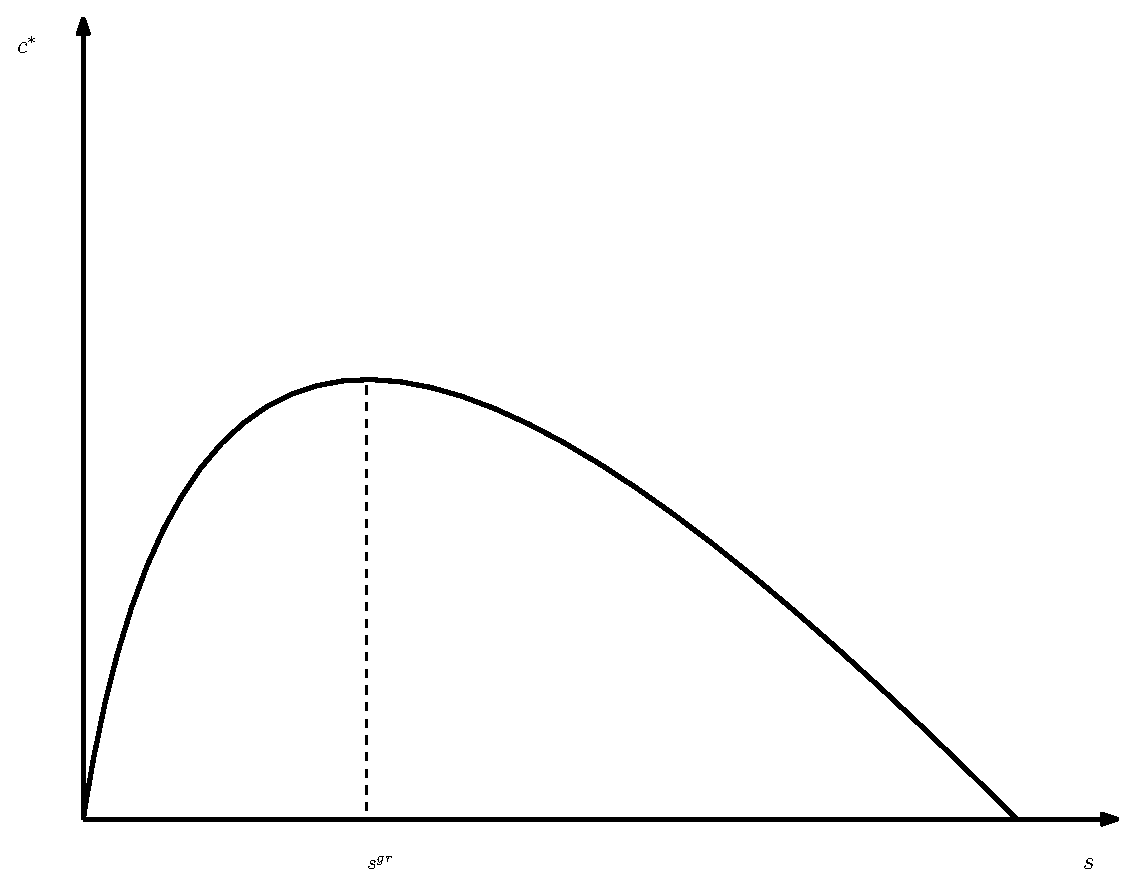
\includegraphics[scale=.4]{solow09.eps}
\label{fig:goldenrule}
\end{figure}
O eixo vertical representa o consumo, enquanto o eixo horizontal a poupança. A taxa de poupança ótima é representada por $s^{gr}$\footnote{Golden rule.}\\

Ainda por uma análise gráfica, a Figura \ref{fig:goldenrule2} mostra porque a regra de ouro deve vigorar. O gráfico apresenta $y_t, i_t$ e $\delta k_t$ contra $k_t$. Isso é, dado o valor de $k_t$ a distância vertical entre $y_t$ e $i_t$ é o consumo $c_t$. Em outras palavras, o estado estacionário é onde $i_t$ cruza $\delta k_t$. Então, o estado estacionário do consumo é dado pela distância vertical de $y_t$ e $i_t$, dado um valor $k^{\ast}$. A regra de outro é o valor da taxa de poupança que maximiza essa distância. Graficamente esse ponto deve ser onde $y_t$ é tangente a curva de $\delta k_t$. Para ser tangente temos que ter $Af'(k_t) = \delta$, isso é , a \textbf{regra de ouro} - a taxa de depreciação do capital sendo igual ao produto marginal do capital.

\begin{figure}[!h]
\centering
\caption{A regra de ouro e a taxa de poupança} \vspace{2ex}
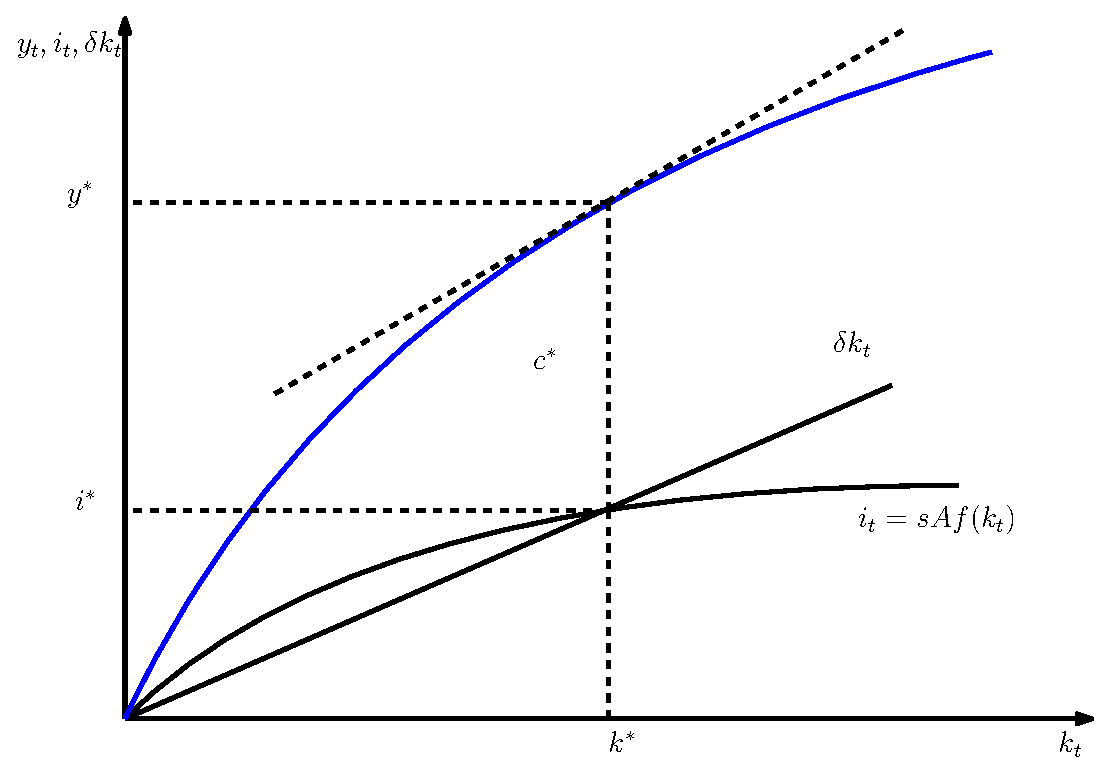
\includegraphics[scale=.6]{solow10.eps}
\label{fig:goldenrule2}
\end{figure}


\end{document}